\section{Casos de Uso}
uwu explicación general
\subsection{Caso de uso I: Detección}
\begin{center}
    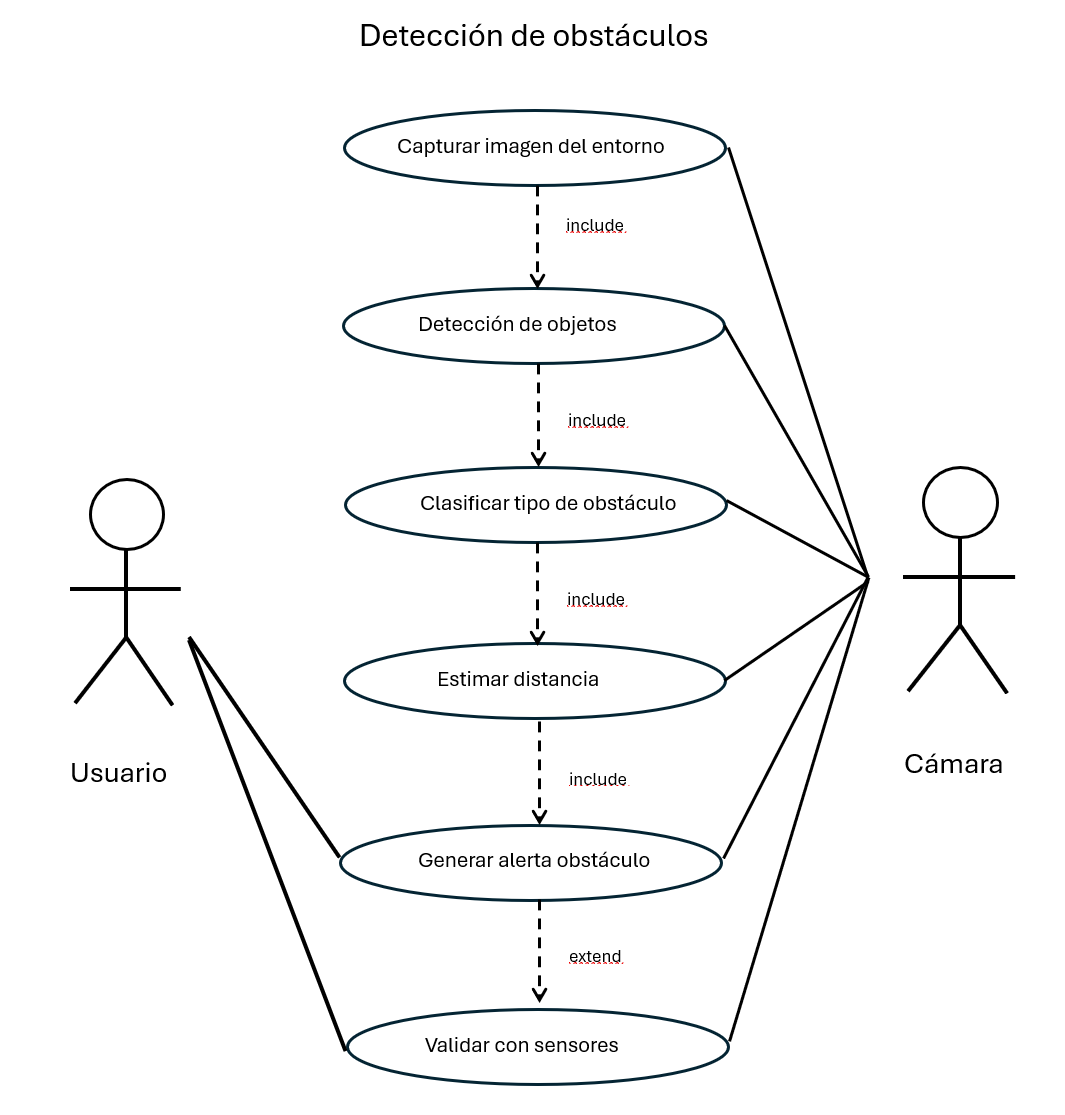
\includegraphics[width=14cm]{Diagramas/DiagDeteccion.png}
\end{center}
Este módulo opera de forma continua y en tiempo real. 

Sus actores son el Usuario (que recibe las alertas) y el actor Cámara / Sensores (que alimenta el sistema con datos del entorno).

Capturar imagen del entorno es el origen del flujo; la cámara toma fotogramas de forma constante y los entrega al pipeline de procesamiento.

Detectar objetos, recibe cada fotograma e identifica todos los elementos presentes: personas, obstáculos, escaleras, automóviles, entre otros. Esta detección es la salida principal que alimenta al módulo de IA.

Clasificar tipo de obstáculo toma las detecciones del modelo y las categoriza según su nivel de riesgo porque un poste estático no es igual de urgente que una persona caminando hacia el usuario.
Estima la distancia al obstáculo, complementa la clasificación usando los datos de sensores de profundidad; sin esta estimación, el sistema no puede determinar qué tan inminente es el peligro.

Generar alerta de obstáculo es el resultado directo: si el obstáculo clasificado supera un umbral de riesgo y se encuentra dentro de cierta distancia, se dispara la alerta hacia el módulo de voz.

Validar con fusión sensorial extiende («extend») el flujo antes de emitir la alerta ya que combina la información visual con los datos de los sensores para reducir falsos positivos. No siempre es necesaria, pero incrementa la confiabilidad del sistema.

\subsection{Caso de uso II: Voz}
\begin{center}
    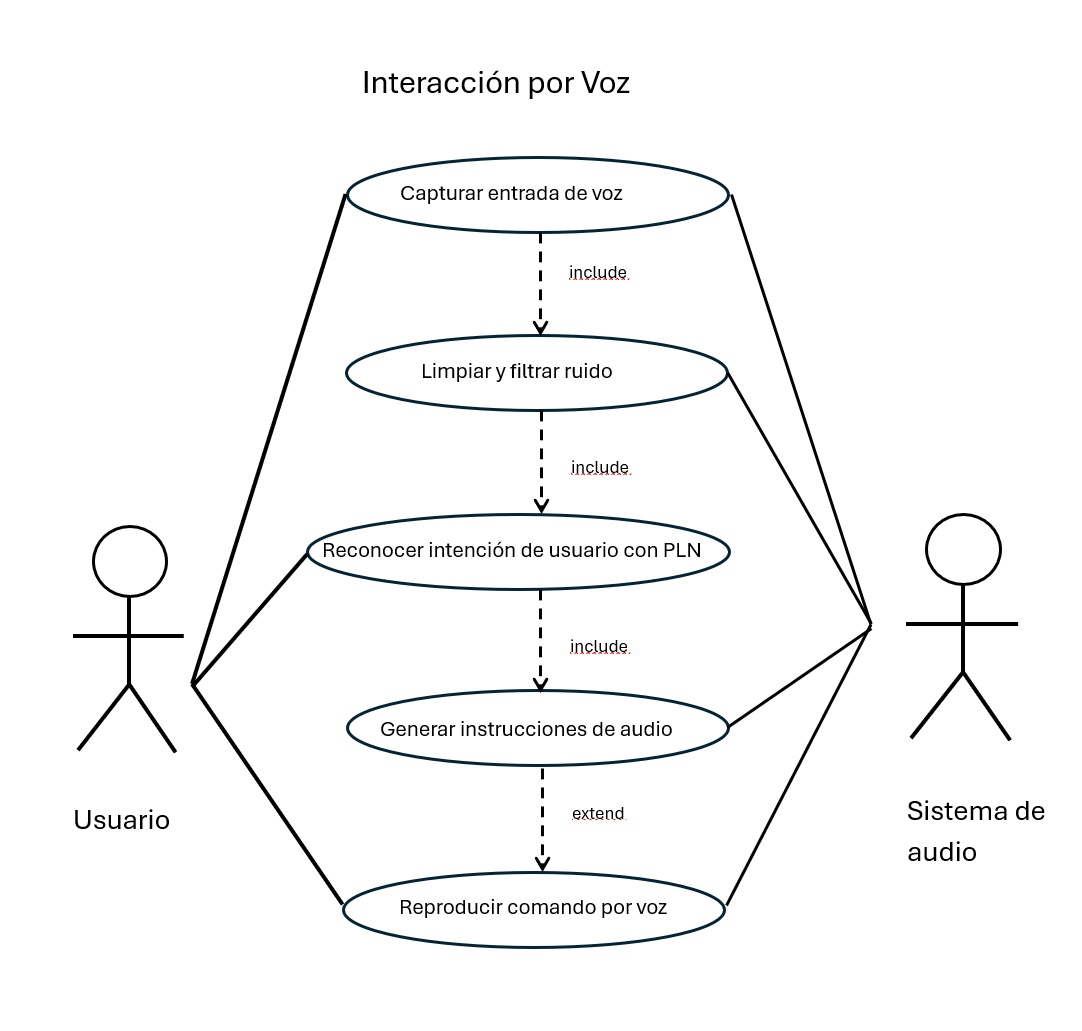
\includegraphics[width=14cm]{Diagramas/DiagVoz.png}
\end{center}
Este módulo es la interfaz principal entre el usuario y el sistema, tanto para entrada (comandos) como para salida (instrucciones y alertas). Sus actores son el Usuario y el Sistema de audio (micrófono y altavoz).

Capturar comando de voz inicia el flujo de entrada; el micrófono detecta que el usuario está hablando y captura el segmento de audio correspondiente.

Filtrar ruido del audio limpia la señal capturada aplicando filtros digitales para eliminar ruido ambiental, viento u otras interferencias que puedan afectar el reconocimiento.

Reconocer intención del usuario interpreta el audio filtrado y lo traduce a una acción concreta dentro del sistema: solicitar un destino, repetir la última instrucción, preguntar la ubicación actual, entre otras.

Generar instrucción de audio toma la respuesta del sistema (ya sea una ruta, una alerta o una confirmación) y la convierte en un mensaje de voz claro y conciso, adaptado al contexto actual del usuario.

Reproducir alerta de voz extiende («extend») el flujo cuando el mensaje generado corresponde a una alerta crítica (obstáculo cercano, cambio de ruta urgente); en esos casos se prioriza la reproducción inmediata por encima de cualquier otra instrucción en cola.
\subsection{Caso de uso III: Navegación}
\begin{center}
    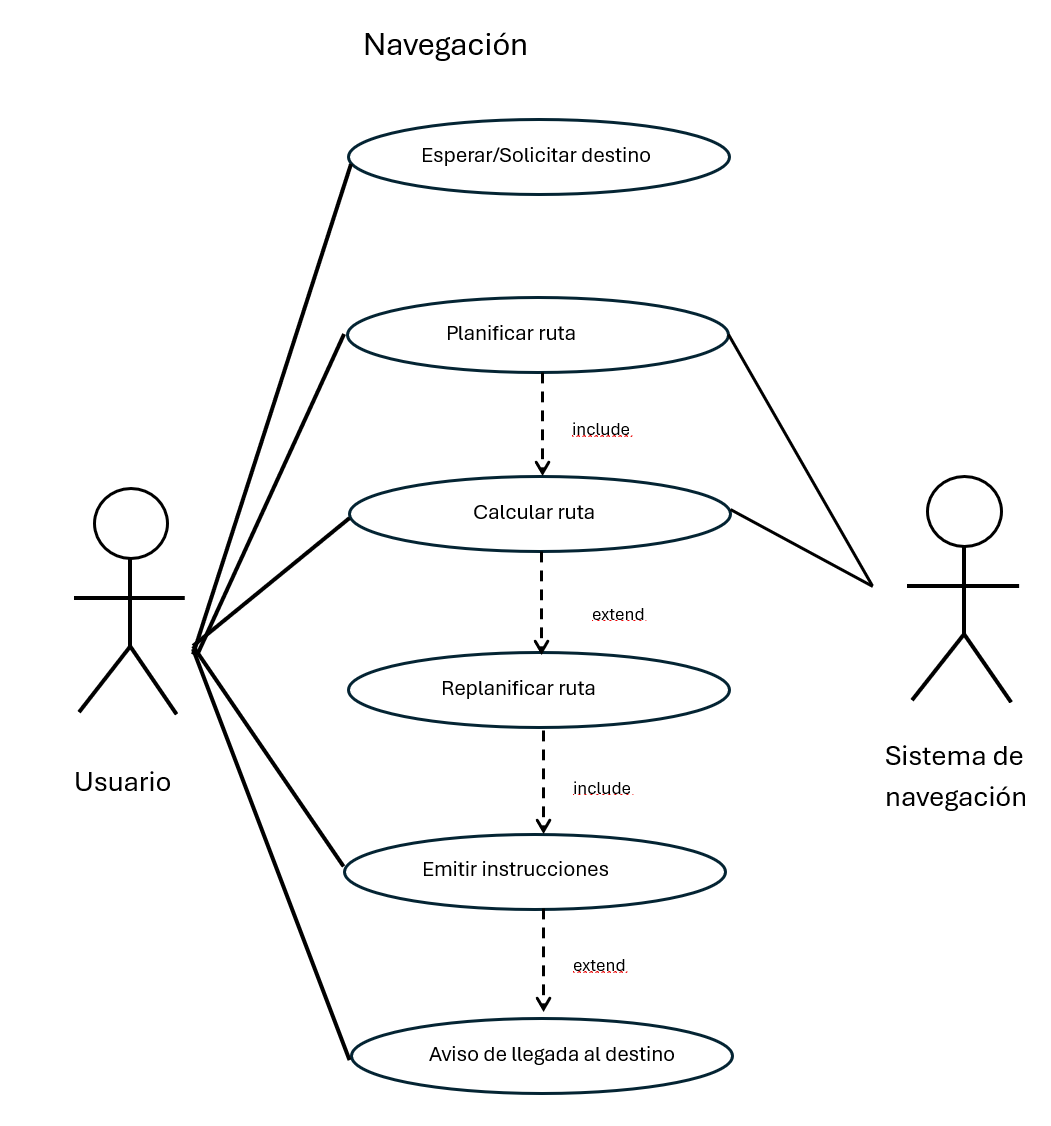
\includegraphics[width=14cm]{Diagramas/DiagNavegacion.png}
\end{center}
Este módulo gestiona el traslado del usuario desde su ubicación actual hasta un destino solicitado. Intervienen dos actores, el Usuario (quien interactúa con el sistema) y el sistema conformado por el módulo de navegación y rutas.

Solicitar destino es el punto de entrada; el usuario indica a dónde quiere ir mediante un comando de voz. A partir de ahí, el sistema ejecuta Planificar ruta global, que se apoya directamente en API Maps para obtener la ubicación actual y basado en la mejor ruta encontrada por el módulo, traza el camino a gran escala considerando calles, distancias y puntos de referencia. Esta relación es un «include» porque la planificación siempre requiere consultar el mapa.

Calcular la ruta se basa en encontrar el mejor camino posible. Para ello, se comparan múltiples rutas y, en cada una, las diferentes posibilidades, eligiendo finalmente la opción más segura.

Re-planificar ruta extiende («extend») al flujo principal cuando el sistema detecta que el camino original ya no es viable, por ejemplo ante un obstáculo imprevisto o un desvío. No ocurre siempre, de ahí la relación de extensión.

Emitir instrucción se incluye («include») en cada segmento de ruta calculado, ya que el sistema siempre debe indicar al usuario qué acción tomar (girar a la derecha, continuar recto, etc.).

Avisar llegada a destino extiende el flujo al final del recorrido; es condicional porque solo se activa cuando la ubicación del usuario coincide con el destino planificado.

\newpage
\begin{center}
    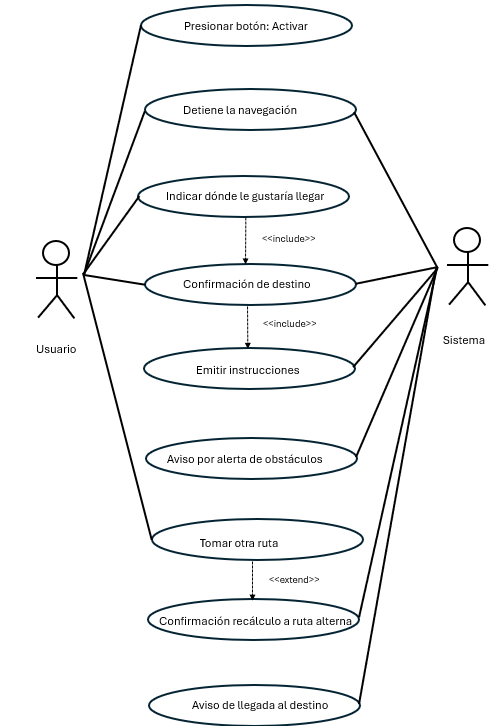
\includegraphics[width=14cm]{Diagramas/DiagCasoUso.png}
\end{center}
Este caso de uso gestiona el traslado del usuario desde su ubicación actual hasta un destino solicitado. Intervienen dos actores: el Usuario (quien interactúa con el sistema) y el Sistema (los lentes).

Indicar dónde le gustaría llegar es el punto de entrada; el usuario comunica su destino al sistema. A partir de ahí, el sistema ejecuta Confirmación de destino, que se apoya en la validación de la dirección para asegurar que el punto final es alcanzable y correcto. Esta relación es un «include» porque la navegación siempre requiere una confirmación del destino antes de proceder.

Emitir instrucciones se incluye («include») obligatoriamente tras la confirmación, ya que el sistema debe guiar al usuario mediante comandos activos durante todo el trayecto. 

El sistema mantiene activo el caso de Aviso por alerta de obstáculos, donde el módulo monitorea el entorno para informar sobre cualquier peligro detectado.

Confirmación recálculo a ruta alterna extiende («extend») al flujo de Tomar otra ruta. Esto ocurre cuando el usuario decide voluntariamente desviarse o el sistema sugiere una modificación; no es un paso obligatorio en todos los viajes, de ahí su relación de extensión.

Finalmente, Aviso de llegada al destino, cierra el ciclo de navegación una vez que el sistema detecta que se ha alcanzado con éxito la ubicación final. El sistema también permite la opción de Detiene la navegación en cualquier punto, otorgando al usuario el control para finalizar el proceso antes de tiempo.